\documentclass[10pt,aspectratio=169,usenames,dvipsnames]{beamer}
\usetheme[numbering=fraction]{metropolis} % Use Metropolis theme

%% adjusting margin
\setbeamersize{text margin left=5mm,text margin right=5mm}

\usepackage{xcolor} % For custom colors
\usepackage{tikz} % For styling enumerate numbers
\usepackage{tcolorbox} % For colored box styling
\usepackage{amsmath, amsfonts, amssymb, amsthm} % Math related
\usepackage{natbib}
\usepackage{appendixnumberbeamer}

% ---------------- %
% color definition %
% ---------------- %
\definecolor{main}{HTML}{23373B}
\definecolor{pink}{RGB}{180, 50, 110}
\definecolor{orange}{HTML}{FF8000}
\definecolor{red}{HTML}{990000}
\definecolor{blue}{HTML}{004C99}
\definecolor{lightgray}{HTML}{E7E7E7}
\definecolor{gray}{RGB}{90, 90, 90}

\newcommand{\pink}[1]{\textcolor{pink}{#1}}
\newcommand{\orange}[1]{\textcolor{orange}{#1}}
\newcommand{\red}[1]{\textcolor{red}{#1}}
\newcommand{\blue}[1]{\textcolor{blue}{#1}}

\setbeamercolor{alerted text}{fg=orange}

% Apply Custom Colors
\setbeamercolor{frametitle}{fg=main, bg=lightgray}
\setbeamercolor{section title}{fg=gray}
\setbeamercolor{title}{fg=main}
\setbeamercolor{structure}{fg=main}
\setbeamercolor{item}{fg=main}

% --------------------------------- %
% enumerate and itemize environment %
% --------------------------------- %
\setbeamertemplate{enumerate item}{%
    {\color{white}\fcolorbox{pink}{pink}{{\arabic{enumi}}}}%
}

\setbeamertemplate{itemize item}{\color{red}\small$\blacktriangleright$}

% --------------------------------- %
% Font: Fira Sans with light weight %
% --------------------------------- %
\usepackage[light,sfdefault]{FiraSans} % Use Fira Sans Light as default sans-serif
\usepackage{FiraMono} % Use Fira Mono for monospaced text
\renewcommand*\familydefault{\sfdefault}
\makeatletter
\def\bfseries@sf{medium}
\def\mdseries@sf{light}
\def\mathfamilydefault{cmss}
\makeatother
\usepackage[T1]{fontenc}
\usepackage{fontawesome}

% --------------------------- %
% Section title page with toc %
% --------------------------- %
\setbeamertemplate{section in toc}[square]
\setbeamertemplate{subsection in toc}[square]
\AtBeginSection[]{
\begin{frame}[noframenumbering]{Outline}
    % \tableofcontents[currentsection]
    \tableofcontents[currentsection, currentsubsection]
\end{frame}
}
\AtBeginSubsection[]{
  \begin{frame}[noframenumbering]{Outline}
    \tableofcontents[currentsection, currentsubsection]
  \end{frame}
}

% ------------ %
% beamerbutton %
% ------------ %
\newcommand{\goto}[2]{\hyperlink{#2}{\beamergotobutton{#1}}}
\newcommand{\return}[2]{\hyperlink{#2}{\beamerreturnbutton{#1}}}
\newcommand{\extgoto}[2]{\href{#2}{\beamergotobutton{#1}}}

\title[Syntax \& Algorithm]{Julia Syntax and Algorithm}
\author[Hui-Jun Chen]{Hui-Jun Chen}
\institute[OSU]{The Ohio State University}
% \date{\today}
\date{\today}
\setbeamertemplate{navigation symbols}{}

\usepackage[cache=true]{minted} % for code chuck and syntax highlighting
\colorlet{verylightgray}{gray!20}
%% shortcuts for julia code chuck
\newminted{julia}{}
\newmintinline{julia}{}
\setmintedinline[julia]{bgcolor=verylightgray}
\setminted[julia]{bgcolor=verylightgray}


\begin{document}

% Title Page
\begin{frame}
    \titlepage
\end{frame}

\section{Basic Julia Usage}
\label{sec:Basic_Julia_Usage}

\begin{frame}\frametitle{THE MOST important coding rules}
\begin{columns}
\label{Quote}
\column{1\linewidth}
\centering
{\Huge \alert{Leggi le leggi}}
\end{columns}

\vspace{2cm}
\begin{center}
    (``Read the manuals'' in Italian)
\end{center}
\end{frame}


\begin{frame}{Resources on Syntax}
\label{slide:Resources_on_Syntax}
    \begin{itemize}
        \item \blue{\href{https://docs.julialang.org/en/v1/manual/getting-started/}{Julia Official Tutorial}}: \tiny \url{https://julialang.org/learning/tutorials/}
        \normalsize
        \item \blue{\href{https://en.wikibooks.org/wiki/Introducing_Julia}{Wikibook on Introducing Julia}}: \tiny{\url{https://en.wikibooks.org/wiki/Introducing_Julia}}
        \normalsize
        \item \blue{\href{https://julia.quantecon.org/intro.html}{QuantEcon w/ Julia}}: \tiny{\url{https://julia.quantecon.org/intro.html}}
        \normalsize
        \item \blue{\href{https://www.youtube.com/watch?v=JYs_94znYy0}{Julia in 100 Seconds}}: \tiny{\url{https://www.youtube.com/watch?v=JYs_94znYy0}}
        \normalsize
    \end{itemize}
\end{frame}

\begin{frame}{The REPL}
\label{slide:The_REPL}
    REPL stands for \textbf{R}ead, \textbf{E}valuate, \textbf{P}rint, and \textbf{L}oops.

    Julia's REPL is the best I have ever seen, includes
    \begin{itemize}
        \item Unicode transformation: type \juliainline{\alpha} and \juliainline{tab} leads to $ \alpha $
        \item Package management: type \juliainline{]} to enter \juliainline{Pkg} mode to \juliainline{add} packages
        \item Manual query: type \juliainline{?} to enter \juliainline{help} mode \& find function manual
        \item Tab completion: type \juliainline{\al} and \juliainline{tab} gives you possible commands
        \item $ \uparrow  $ / $ \downarrow  $: up/down arrow key cycle through executed command history
    \end{itemize}

\end{frame}

\begin{frame}{The Language: Good and Bad}
\label{slide:The_Language__Good_and_Bad}

Julia language is designed with scientific computing in mind, and thus

\begin{itemize}
    \item Unicode variable: directly use $ \alpha $ as variable, not \juliainline{alpha}.
    \item Multiple dispatch: multiple ``methods'' in one function for input types
    \item Type system: use \juliainline{struct} to build custom types ($\approx$ but $\neq$ OOP)
\end{itemize}

But also have some weird behavior that I am not used to:

\begin{itemize}
    \item \blue{\href{https://craftofcoding.wordpress.com/2021/02/12/what-i-really-dislike-about-julia-its-scope/}{Weird scope}}: variables defined inside loops (\juliainline{while}, \juliainline{for}) are \textbf{local}.
    \item Speed needs discipline: \textbf{well-written} code v.s. \textbf{sloppy-written} code
    \item Memory usage: might directly crash the Julia session ($\because$ LLVM?)
\end{itemize}

Best practice? \hspace{2.5cm} Still Searching...

\end{frame}

\section{Syntax}
\label{sec:Syntax}

\begin{frame}[fragile]{Syntax: generating a grid}
\label{slide:Syntax__generating_a_grid}

\begin{itemize}
    \item Usually the Macro coding starts with the grids of choice variables.
    \item A grid is a finite sample of continuous choice variable.
    \item Key to construct a grid is the \juliainline{collect} and \juliainline{range} function.
    \item \juliainline{range} syntax requires \juliainline{start} pt, \juliainline{stop} pt and \juliainline{length} of this grid
    \item \juliainline{collect} then ``collect'' this \juliainline{range} object into an array.
\end{itemize}


\begin{juliacode}
    cnum = 100
    lnum = 100
    cgrid = collect( range( 0.01, 10.0, length = cnum ) )
    lgrid = collect( range( 0.01, 1.0, length = lnum ) )
\end{juliacode}
\end{frame}

\begin{frame}[fragile]{Syntax: Array manipulation}
\label{slide:Syntax__Array_manipulation}
To get one element of a grid, we use \juliainline{[]} syntax.
\begin{juliacode}
    cval = cgrid[1] # get the first element of cgrid
    lval = lgrid[5] # get the fifth element of lgrid
\end{juliacode}
To create an array, you can use manual or automatical way.
\begin{juliacode}
    # manually type all the elements
    a = [1.0, 2.0, 3.0, 4.0, 5.0 ]
    # automatically generate an "empty" array
    #               type    dim empty  row   column
    utility = Array{Float64, 2}(undef, cnum, lnum)
    utility = zeros(cnum, lnum) # zero array
    utility = ones(cnum, lnum) # one array
\end{juliacode}

\end{frame}


\begin{frame}[fragile]{Syntax: \juliainline{for} loop}
\label{slide:Syntax___mintinline_julia__for__loop}

To calculate the utility value at each $ (C, l) $ bundle, use \juliainline{for} loop

\begin{juliacode}
    utility = Array{Float64, 2}(undef, cnum, lnum)
    for indl in 1:1:lnum
        # get the each value in leisure grid
        lval = lgrid[indl]
        for indc in 1:1:cnum
            # get the each value in consumption grid
            cval = cgrid[indc]
            # log utility in both c and l
            utility[indc, indl] = log(cval) + log(lval)
        end
    end
\end{juliacode}
\return{Gov spending}{slide:Grid_search__easiest_method_possible}
\end{frame}

\begin{frame}[fragile]{Syntax: 3-D plotting}
\label{slide:Syntax__3_D_plotting}

Install \juliainline{Plots} and \juliainline{PyPlot} by typing \juliainline{]} and type \juliainline{add Plots PyPlot}

Plot the \juliainline{utility} array by

\begin{juliacode}
    using Plots; pyplot();
    surface(cgrid, lgrid, utility)  # 3-D figure
\end{juliacode}

\begin{center}
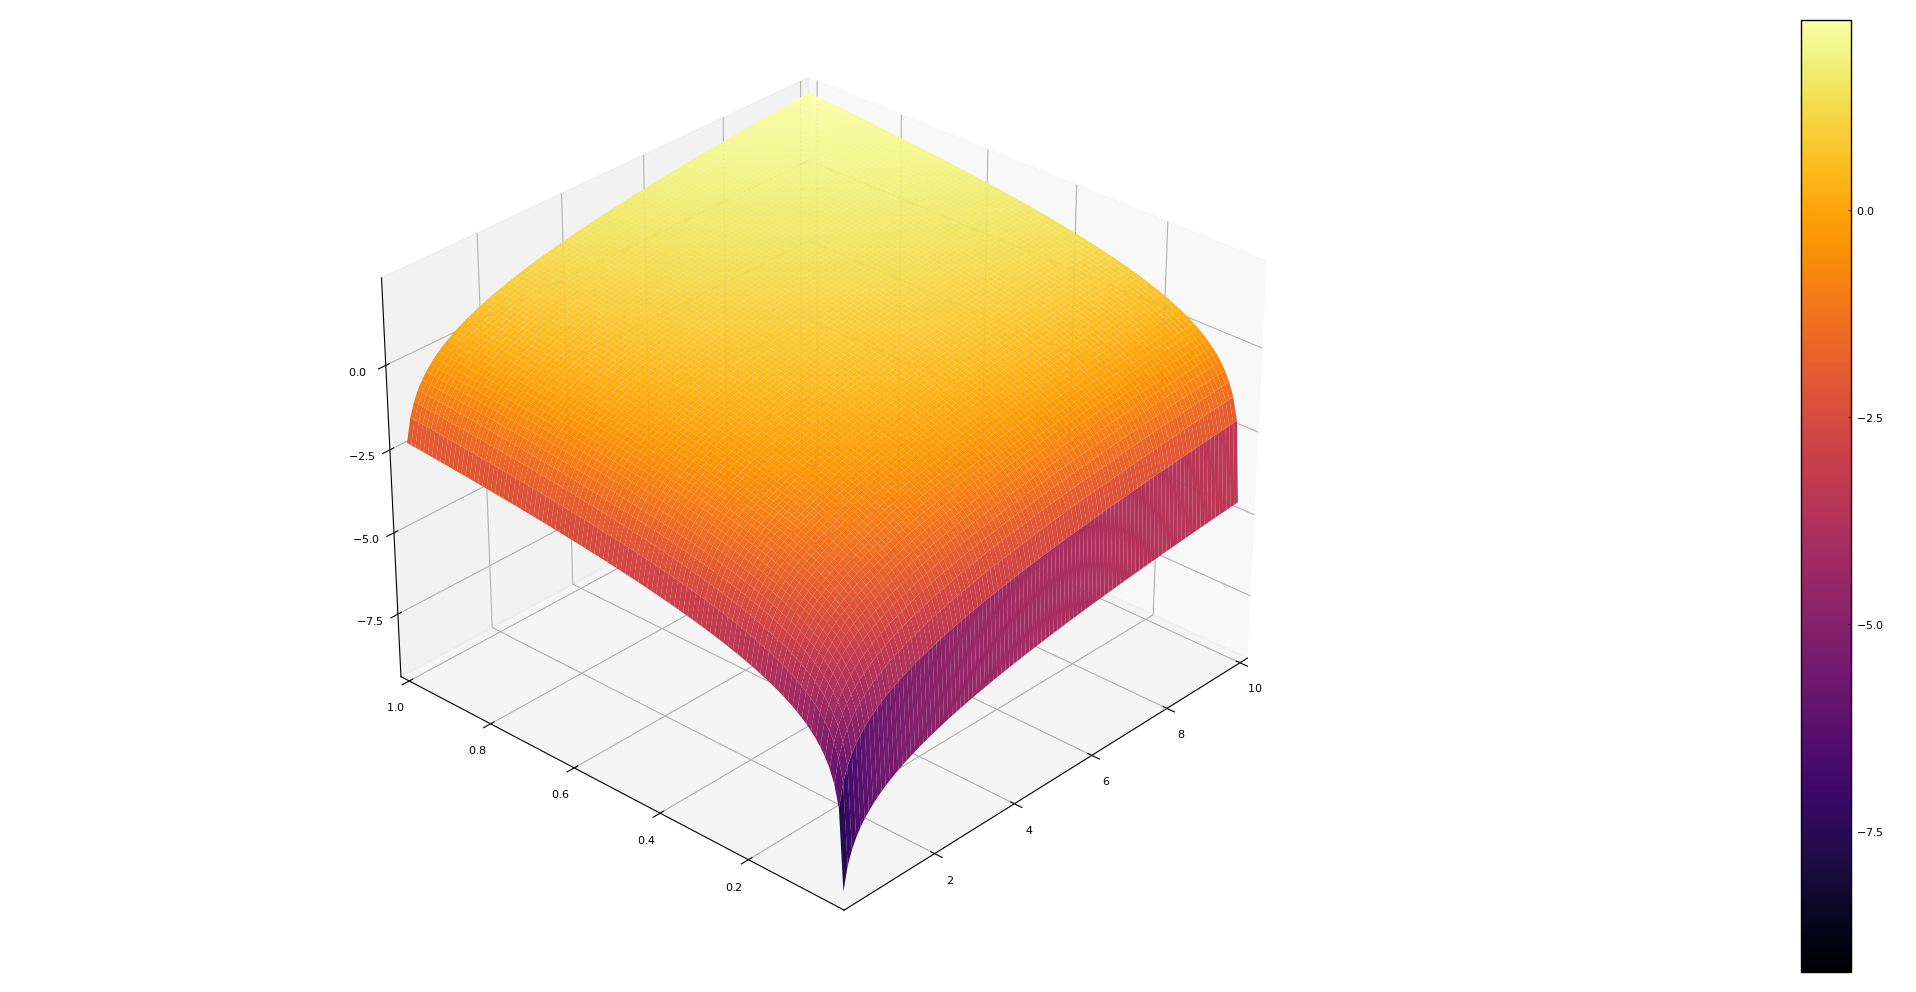
\includegraphics[width=0.6\textwidth]{./figures/utility.png}
\end{center}
\end{frame}

\begin{frame}[fragile]{Syntax: contour plotting}
\label{slide:Syntax__contour_plotting}

\begin{juliacode}
    using Plots; pyplot();
    contour(cgrid, lgrid, utility)  # contour figure
\end{juliacode}

\begin{center}
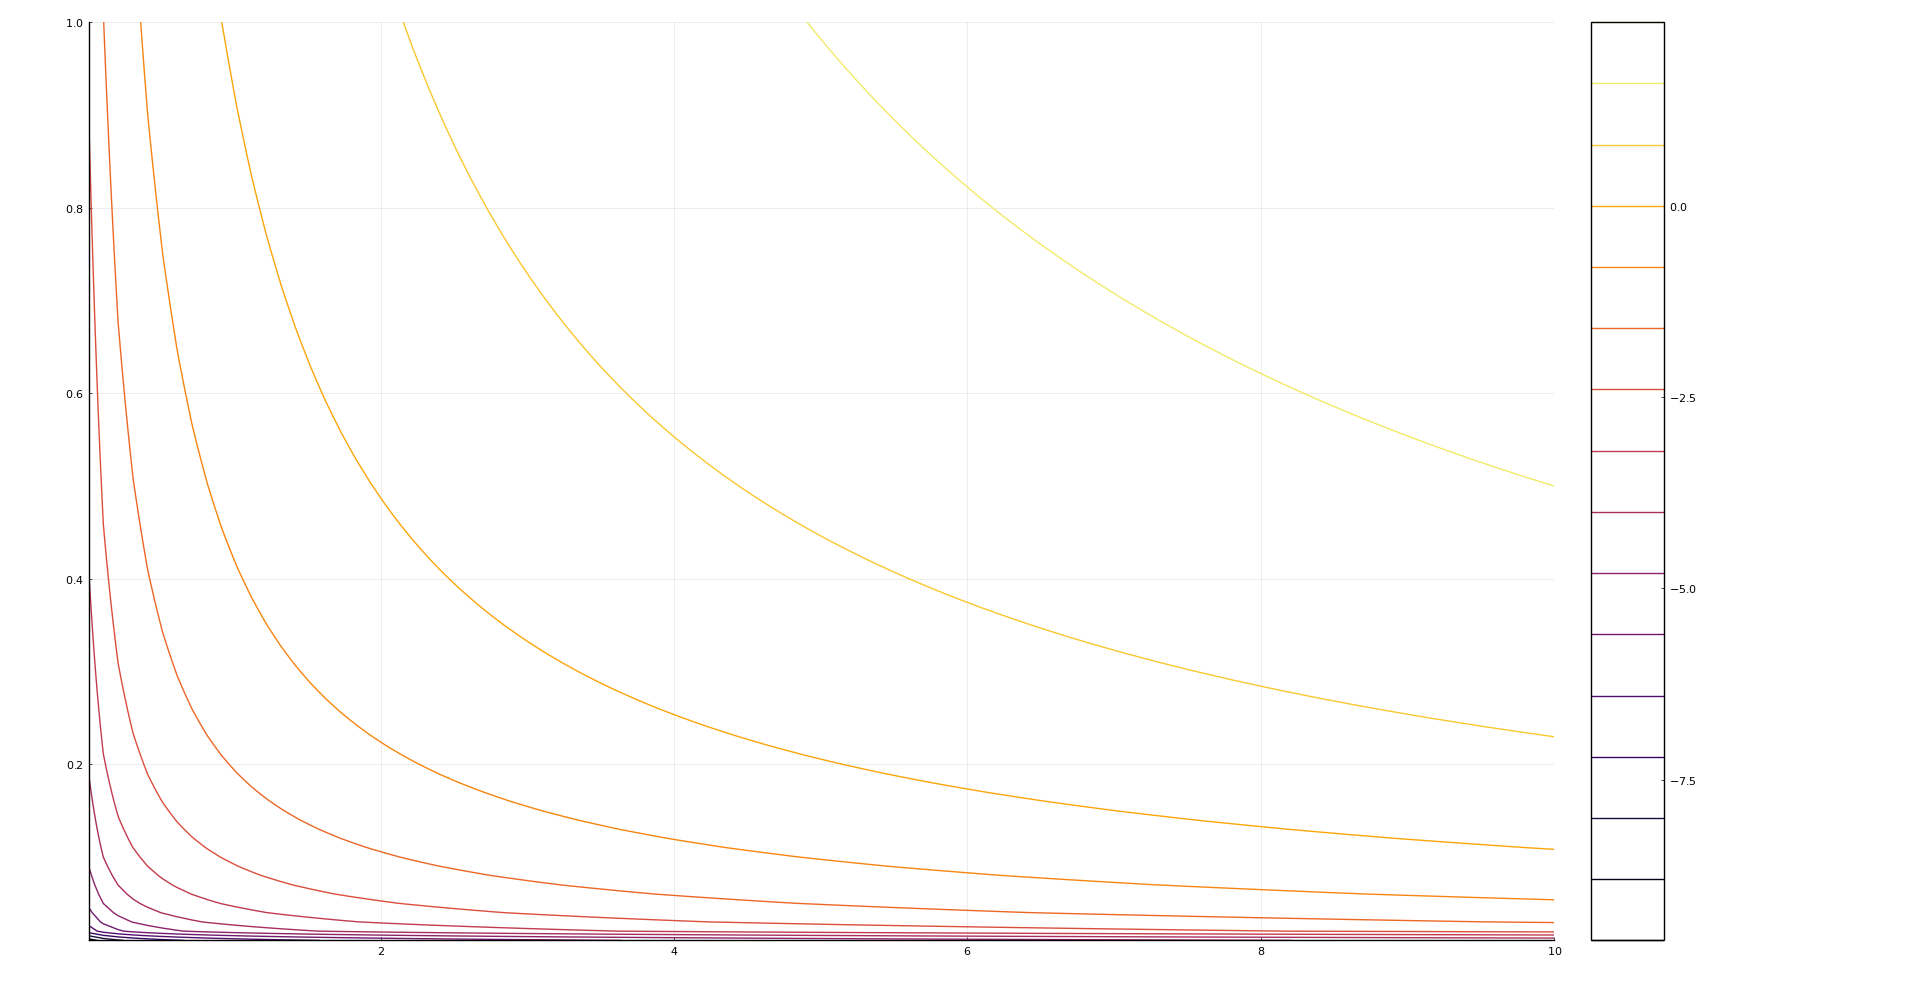
\includegraphics[width=0.8\textwidth]{./figures/utility_contour.png}
\end{center}

\end{frame}

\begin{frame}[fragile]{Syntax: \juliainline{println} print something out}
\label{slide:Syntax___mintinline_julia__println__print_something_out}

To show some info inside the \juliainline{for} loop, \juliainline{println} is a convenient tool.

If you want to know what $ (C, l) $ bundle leads to $ U(C, l) = 0.0 $,

\begin{juliacode}
    for indl in 1:1:lnum
        for indc in 1:1:cnum
            # the abs of u is close enough to 0.0
            if abs(utility[indc, indl]) < 1e-2
            # '$': string interpolation (IMO inefficient)
                println("U ~ 0 at (C, l) = ($indc, $indl)")
            end
        end
    end
\end{juliacode}
\juliainline{println} v.s. \juliainline{print}: \juliainline{println} add additional \juliainline{\n}
\end{frame}


\begin{frame}[fragile]{Syntax: \juliainline{while} loop}
\label{slide:Syntax___mintinline_julia__while__loop}
    \juliainline{while} loop mostly used when iteration only hault in some conditions.

    In my experience it is mostly used if something needs convergence.

    The following code is \textbf{NOT} an efficient way to find minimum location.

    (should use \juliainline{argmin} for \juliainline{minimum} and \juliainline{argmax} for \juliainline{maximum})

\begin{juliacode}
    dist = 1.0; iter = 0;
    while (dist > 1e-2)
        iter += 1 # same as "iter = iter + 1"
        indc = rand(1:1:cnum); indl = rand(1:1:lnum)
        dist = utility[indc, indl] - minimum(utility)
        if (dist < 1e-2)
            println("Find minimum at ($indc, $indl)")
            println("Iterates $iter times")
        end
    end
\end{juliacode}

\end{frame}

\begin{frame}[fragile]{Syntax: Rounding}
\label{slide:Syntax__Rounding}
    Mostly for exam / standardization purpose.

    \begin{juliacode}
        round(pi)               # 3.0
        round(pi, digits = 1)   # 3.1
        round(pi, digits = 2)   # 3.14
        round(pi, digits = 3)   # 3.142
        round(pi, digits = 4)   # 3.1416
        round(pi, digits = 5)   # 3.14159
    \end{juliacode}
\end{frame}

\section{Laffer curve}
\label{sec:Laffer_curve}

\begin{frame}{Application: Laffer curve}
\label{slide:Application__Laffer_curve}

There are going to be two applications for Julia syntax learned:
\begin{enumerate}
    \item Laffer curve in distorting taxes, and
    \item Government spending in CRRA utility function.
\end{enumerate}

Recall that $ Y = z N^{d} $ implies labor supply $ N^{s}(t) $ equals to

%
\begin{equation}
\label{eq:laborSupplyTaxRate}
    N^{s}(t) = 1 - l = \frac{1}{2} - \frac{\pi}{2(1-t)}
,\end{equation}
%
and the total tax revenue is given by
%
\begin{equation}
\label{eq:govTaxRevenue}
    R(t) = w t N^{s}(t)
.\end{equation}
%
In equilibrium $ w = z = 1 $, so $ \pi = z N^{d} - w N^{d} = 0 $, so this question is trivial...

\end{frame}

\begin{frame}{Laffer curve in Cobb-Douglas Production Function}
\label{slide:Laffer_curve_in_Cobb_Douglas_Production_Function}
Assume $ Y = z N^{a} $, where $ a < 1 $, so firm's problem leads to
%
\begin{align}
    w(N)
        & = MPN = z a N^{a-1},
    \\
    \pi(N)
        & = Y - wN = z (1-a) N^{a},
\end{align}
%
and recall $ MRS_{l, C} = w(1-t) $ and binding BC $ C = w(1-t)N + \pi $, so
%
\begin{align}
    MRS_{l, C} = \frac{C}{l}
        & = \frac{w (1-t) N + \pi}{l} = w(1-t)
    \\
        & = \frac{w(N) (1-t) N + \pi(N)}{(1-N)} = w(N)(1-t)
\end{align}
%
expands, we get a monster:
%
\begin{equation}
    \begin{split}
        \frac{z a N^{a-1}(1-t)N + z (1-a) N^{a}}{ 1-N}
            & = z a N^{a-1} (1-t)
        \\
    \end{split}
\end{equation}
%
\end{frame}

\begin{frame}{Laffer curve in Cobb-Douglas Production Function (cont.)}
\label{slide:Laffer_curve_in_Cobb_Douglas_Production_Function__cont__}
    But not too bad, because you realize:
    %
    \begin{align}
        \text{Common } N: \quad
            & \frac{z a \red{N^{a-1}}(1-t)\red{N} + z (1-a) N^{a}}{ 1-N} = z a N^{a-1} (1-t)
        \\
        \text{Common } z N^{a}: \quad
            & \frac{\red{z} a \red{N^{a}}(1-t) + \red{z} (1-a) \red{N^{a}}}{ 1-N} = z a N^{a-1} (1-t)
        \\
        \text{Erase } z N^{a-1}: \quad
            & \frac{\blue{z N^{a}} [a (1-t) + 1-a]}{1-N} = \blue{z} a (1-t) \blue{N^{a-1}}
        \\
        \text{Divide } [\cdot]: \quad
            & \frac{N \blue{[a (1-t) + 1-a]}}{1-N} = a (1-t)
        \\
            & \frac{N}{1-N} = \frac{a(1-t)}{a(1-t) + 1-a} \equiv A(t)
        \\
            & N = A(1-N) = A - AN
        \\
            & (1+A)N = A \Rightarrow N(t) = \frac{A(t)}{1+A(t)}
    \end{align}
    %
\end{frame}

\begin{frame}[fragile]{Laffer curve in Julia}
\label{slide:Laffer_curve_in_Julia}
\begin{juliacode}
    a = 0.33; tnum = 1000
    tgrid = collect( range(0.01, 0.99, length = tnum) )
    Gvec = Array{Float64, 1}(undef, tnum)
    for indt = 1:1:tnum
        t = tgrid[indt]
        A = ( a*(1-t) ) / ( a*(1-t) + 1 - a )
        N = A / (1 + A)
        w = a*N^(a-1)
        Gvec[indt] = w * t * N
    end
    Gmax = maximum(Gvec); tmax = tgrid[argmax(Gvec)];
    println("G* = $Gmax; t* = $tmax")
\end{juliacode}
\end{frame}

\begin{frame}[fragile]{Laffer curve in Julia (cont.)}
\label{slide:Laffer_curve_in_Julia__cont__}
\begin{juliacode}
    using Plots; pyplot()
    plot(tgrid, Gvec, label = "G")
\end{juliacode}
\begin{center}
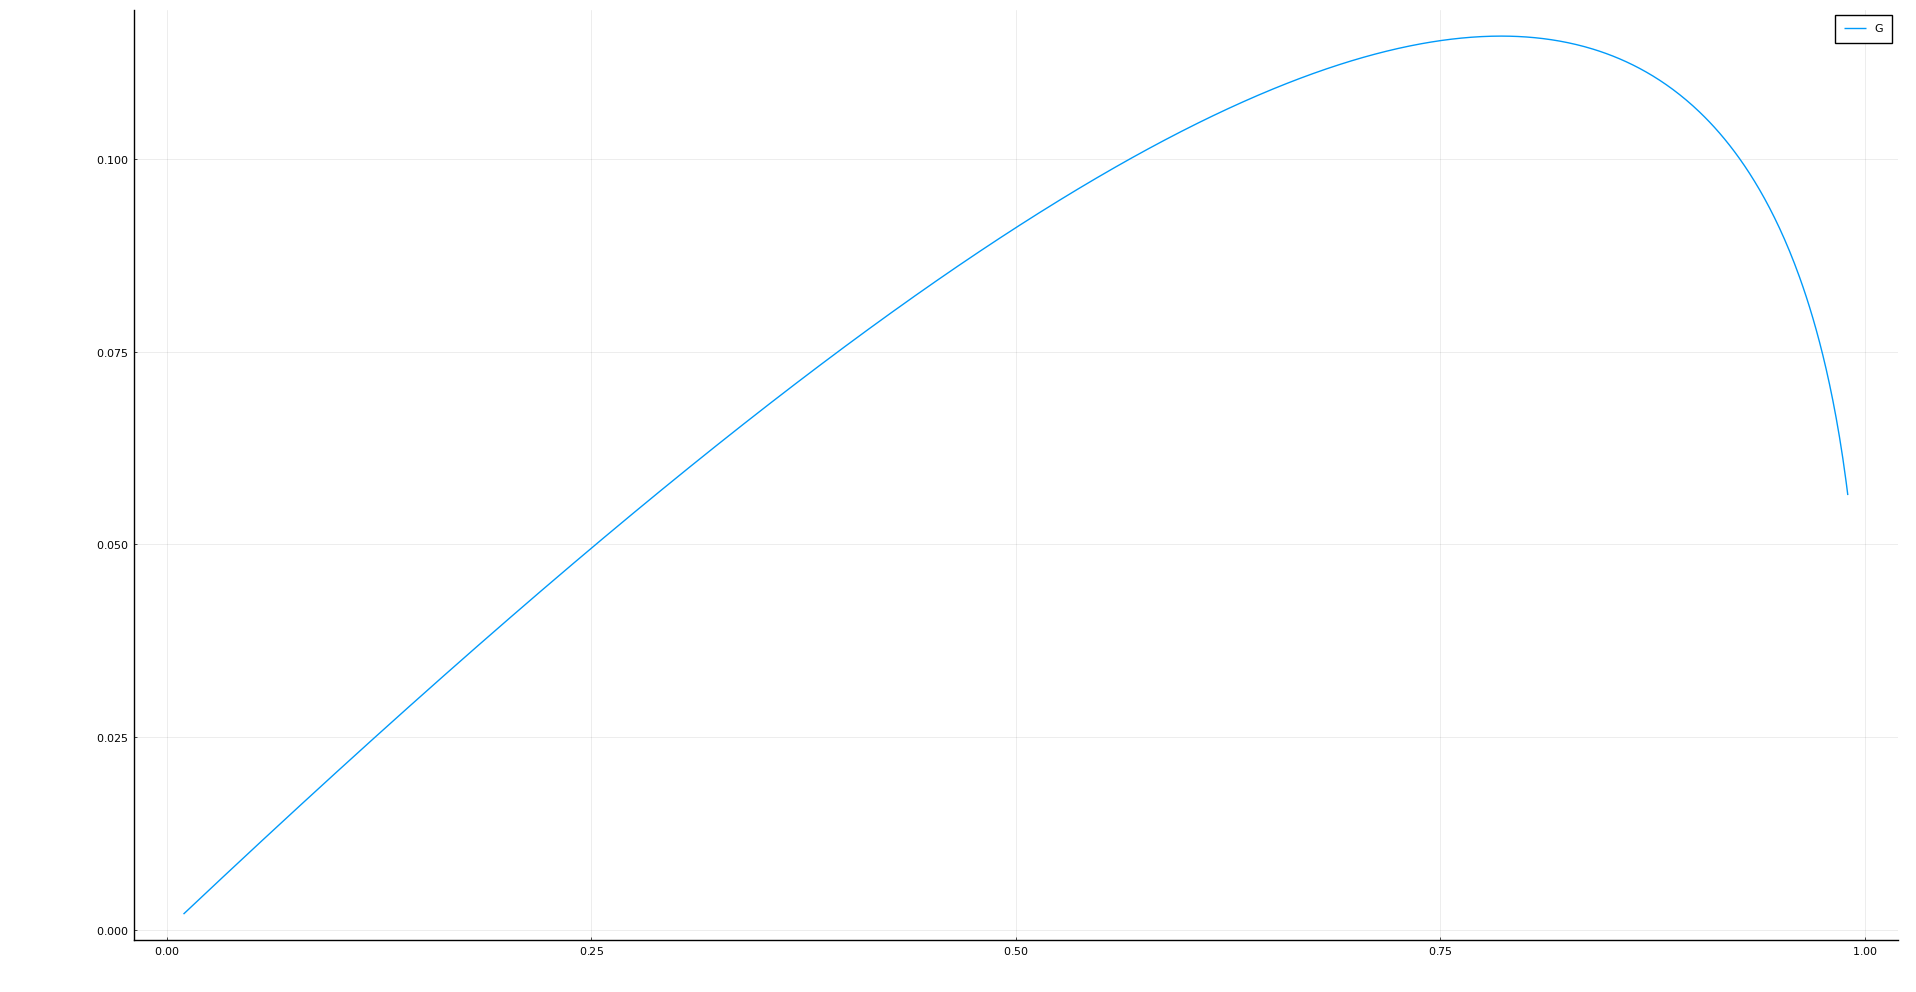
\includegraphics[width=.7\textwidth]{./figures/lafferCurve.png}
\end{center}
\end{frame}


\section{Gov Spending}
\label{sec:Gov_Spending}

\begin{frame}[fragile]{Grid search}
\label{slide:Grid_search__easiest_method_possible}
    Just calculate value \textbf{on} the grid points! Like \goto{for loop}{slide:Syntax___mintinline_julia__for__loop} slide

    Recall the formula with gov spending:

    %
    \begin{equation}
    \label{eq:govspendingQ}
        \max_{l} \quad \frac{(z ( 1-l )^{1-\alpha} - G)^{1-b}}{1-b} + \frac{l^{1-d}}{1-d}
    .\end{equation}
    %
    We want to solve $ l(z, G) $, but how to choose the \juliainline{Ggrid}?

    From the FOC we know
    %
    \begin{equation}
    \label{eq:govspendingQFOC}
        G = F( l ) = z( 1-l )^{1-\alpha} -
            \left[
                \frac{l^{-d}}{( 1-\alpha )z( 1-l )^{-\alpha}}
            \right]^{-\frac{1}{b}}
    .\end{equation}
    %

    Our first step starts with generating a TFP grid:
\begin{juliacode}
    znum = 100
    zgrid = collect( range( 0.8, 1.2, length = znum ) )
\end{juliacode}
\end{frame}

\begin{frame}[fragile]{Grid search: preperation}
\label{slide:Grid_search___preperation}

We want to find the upper/lower bound of \juliainline{Ggrid}:
\begin{juliacode}
    a = 1/2; b = 2; d = 3/2;
    GovFOC(z, l) = z*(1-l)^(1-a) - # line continuation!
        ( (l^(-d)) / ( (1-a)*z*(1-l)^(-a) ) )^(-1/b)
    # upper & lower bound of Ggrid
    Gbound = Array{Float64, 2}(undef, znum, 2)
    for indz = 1:1:znum
        zval = zgrid[indz]
        Gbound[indz, 1] = GovFOC(zval, 0.99) # lower bound
        Gbound[indz, 2] = GovFOC(zval, 0.01) # upper bound
    end
\end{juliacode}

\end{frame}

\begin{frame}[fragile]{Grid search: preperation (cont.)}
\label{slide:Grid_search__preperation__cont__}

\begin{juliacode}
    # lower bound should higher than 0.01
    Glow = max(0.0, minimum(Gbound))
    Ghigh = maximum(Gbound)
    # build Ggrid
    Gnum = 100
    Ggrid = collect( range( Glow, Ghigh, length = Gnum ) )
    # build lgrid
    lnum = 100
    lgrid = collect( range( 0.01, 1.0, length = lnum ) )
\end{juliacode}

and then find the optimal leisure using the value on this grid:

\end{frame}


\begin{frame}[fragile]{Grid search: structure}
\label{slide:Grid_search__structure}
\begin{juliacode}
    a = 1/2; b = 2; d = 3/2;
    # define implicit utility function
    utility(l, z, G) = ( ( z*(1-l)^(1-a) - G )^(1-b) ) /
                        ( 1-b ) +
                        ( l^(1-d) ) / (1-d)
    # Array for storage
    ## for temporary storage
    uvec = Array{Float64, 1}(undef, lnum)
    ## for optimal utility value
    ustar = Array{Float64, 2}(undef, znum, Gnum)
    ## for optimal leisure given z, G
    lstar = Array{Float64, 2}(undef, znum, Gnum)
\end{juliacode}
\end{frame}

\begin{frame}[fragile]{Grid search: structure (cont.)}
\label{slide:Grid_search__structure__cont__}
\begin{juliacode}
    for indG = 1:1:Gnum
        Gval = Ggrid[indG]
        for indz = 1:1:znum
            zval = zgrid[indz]
            for indl = 1:1:lnum
                lval = lgrid[indl]
                cval = zval*(1-lval)^(1-a) - Gval
                uvec[indl] = ( cval < 0.0 ? -Inf :
                                utility(lval, zval, Gval) )
            end
            ustar[indz, indG] = maximum(uvec)
        end
    end
\end{juliacode}

\end{frame}

\begin{frame}[fragile]{Grid search: analysis}
\label{slide:Grid_search__analysis}
Notice that in previous slide, I check whether \juliainline{cval < 0.0}

and also we find the highest utility and the corresponding $ (z, G) $ value by
\begin{juliacode}
    umax = maximum(ustar)
    zloc = argmax(ustar)[1]
    Gloc = argmax(ustar)[2]
    zmax = zgrid[zloc]
    Gmax = Ggrid[Gloc]
\end{juliacode}

But if you plot you will see that the plot is slightly ``off'':
\begin{juliacode}
    using Plots; pyplot()
    surface(zgrid, Ggrid, ustar)
\end{juliacode}

$ \because $ large negative point that drag down the scale of every point.

\end{frame}

\begin{frame}{grid search: misleading figure}
\label{slide:grid_search__misleading_figure}
    \includegraphics[width=\textwidth]{./figures/utilitygov_wrong.png}
\end{frame}

\begin{frame}[fragile]{Grid search: revising (erase \juliainline{uval < -30.0})}
\label{slide:Grid_search__structure__cont__}
\begin{juliacode}
    for indG = 1:1:Gnum
        Gval = Ggrid[indG]
        for indz = 1:1:znum
            zval = zgrid[indz]
            for indl = 1:1:lnum
                lval = lgrid[indl]
                cval = zval*(1-lval)^(1-a) - Gval
                uval = utility(lval, zval, Gval)
                uvec[indl] = ( (cval < 0.0 || uval < -30.0)
                                ? -Inf : uval )
            end
            ustar[indz, indG] = maximum(uvec)
        end
    end
\end{juliacode}

\end{frame}

\begin{frame}{Grid search: better figure}
\label{slide:grid_search__better_figure}
    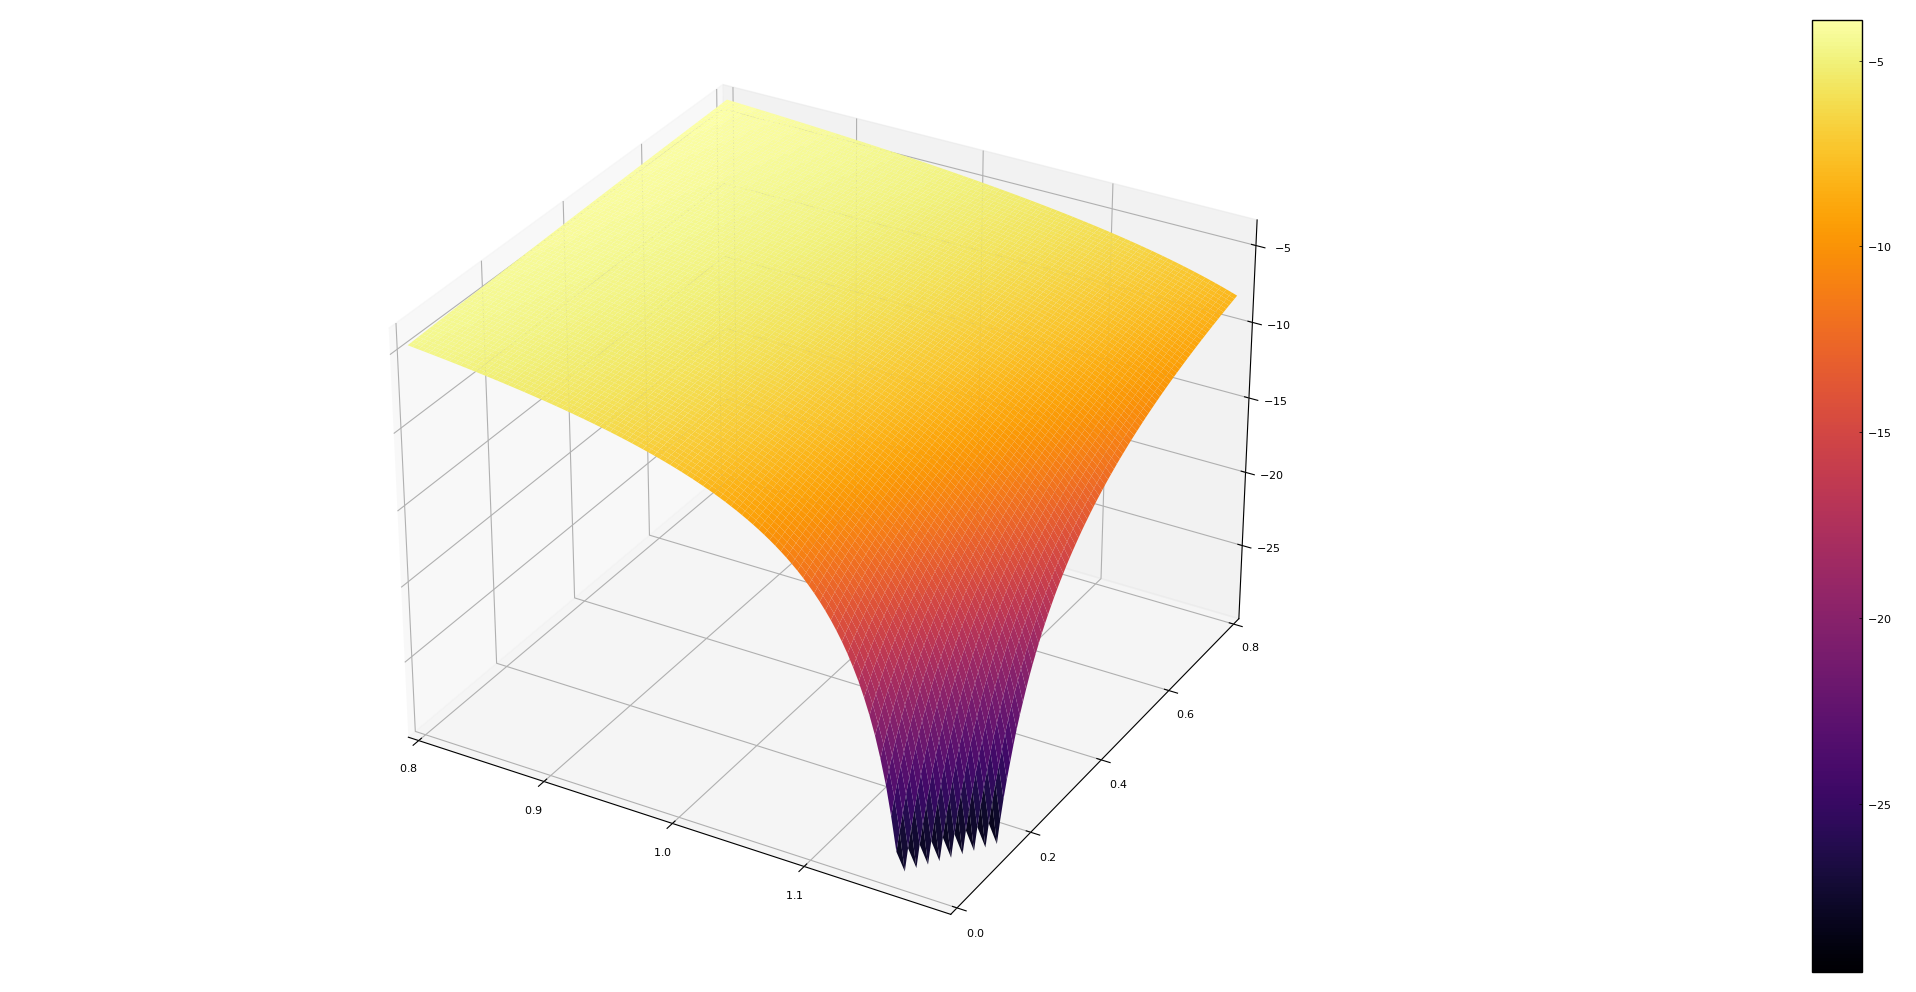
\includegraphics[width=\textwidth]{./figures/utilitygov_correct.png}
\end{frame}

\begin{frame}[fragile]{Grid search: Can we do better?}
\label{slide:Grid_search__Can_we_do_better_}
    All of the \juliainline{-Inf} stuff we are assigning manually is because $ C < 0 $.

    Recall that $ C = Y - G $, and thus for $ C \ge 0 $, $ Y - G \ge 0 \Rightarrow Y > G $.

\begin{juliacode}
    ymat = Array{Float64, 2}(undef, znum, lnum)
    for indl = 1:1:lnum
        lval = lgrid[indl]
        for indz = 1:1:znum
            zval = zgrid[indz]
            ymat[indz, indl] = zval * (1-lval)^(1-a)
        end
    end
    ymin = minimum(ymat)
\end{juliacode}

You will get $ min(y) = 0.081 $, which means that if you choose the \juliainline{Ghigh = 0.08}, $ C > 0, \forall z, G $ assigned.

\end{frame}

\begin{frame}[fragile]{Grid search: do better}
\label{slide:Grid_search__do_better}

\begin{juliacode}
    # lower bound should higher than 0.01
    Glow = 0.0
    Ghigh = 0.08
    # build Ggrid
    Gnum = 100
    Ggrid = collect( range( Glow, Ghigh, length = Gnum ) )
    # build lgrid
    lnum = 100
    lgrid = collect( range( 0.01, 0.99, length = lnum ) )
\end{juliacode}

and then find the optimal leisure using the value on this grid:

\end{frame}

\begin{frame}[fragile]{Grid search: do better (cont.)}
\label{slide:Grid_search__do_better__cont_}

\begin{juliacode}
    for indG = 1:1:Gnum
        Gval = Ggrid[indG]
        for indz = 1:1:znum
            zval = zgrid[indz]
            for indl = 1:1:lnum
                lval = lgrid[indl]
                cval = zval*(1-lval)^(1-a) - Gval
                uvec[indl] = utility(lval, zval, Gval)
            end
            ustar[indz, indG] = maximum(uvec)
        end
    end
\end{juliacode}


\end{frame}

\begin{frame}{Grid search: better figure}
\label{slide:grid_search__better_figure}
    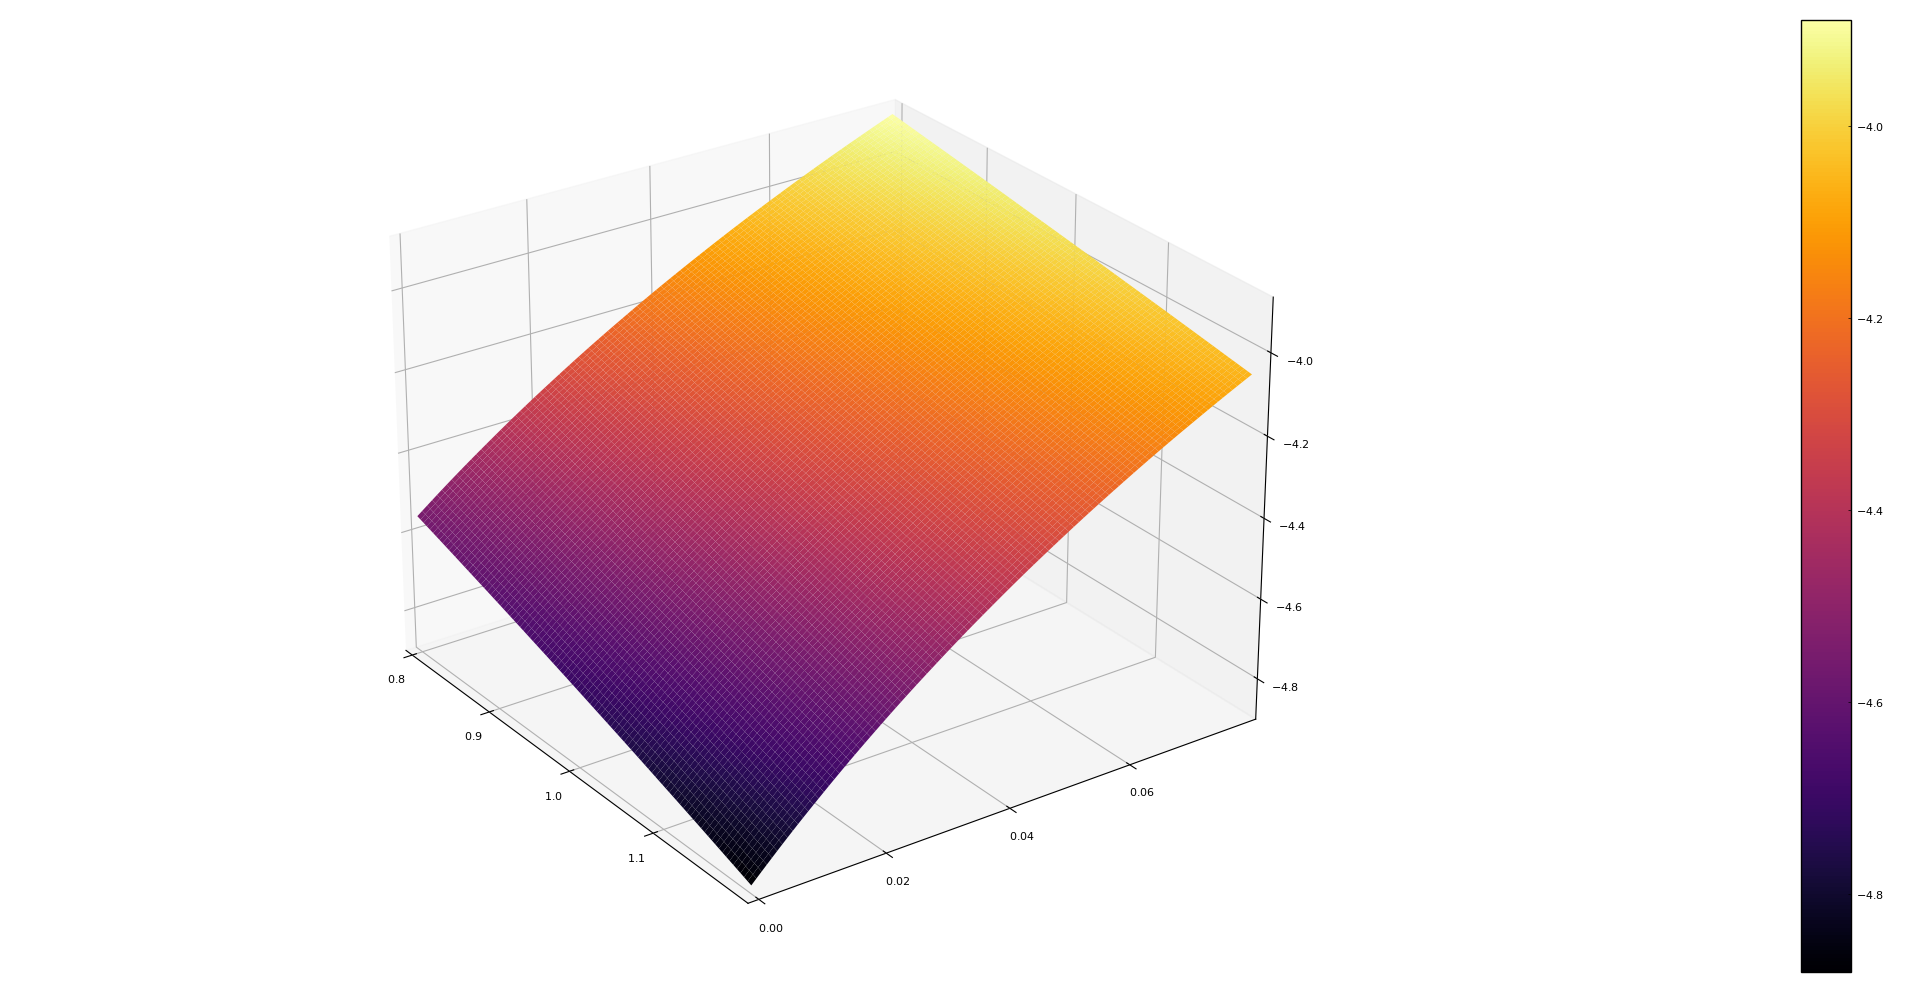
\includegraphics[width=\textwidth]{./figures/utilitygov_better.png}
\end{frame}

\begin{frame}{Grid search method: additional details}
\label{slide:Grid_search_method__additional_details}

Calculate on the grid point $ \Rightarrow  $ result are correct but speed is slow.

Notice that when you choose the grid points, better to avoid some value:

\begin{example}
When I create \juliainline{cgrid} and \juliainline{lgrid}, I avoid the start point of $ 0.0 $, but $ 0.01 $, since $ log(0.0) = \infty $.
\end{example}

In general, if theoretical range, say leisure, is $ [0, 1] $, then it is safe to build a grid from $ [0.01, 0.99] $.

\end{frame}

% \section{Appendix}
% \label{sec:Appendix}
%
% \appendix
% \begin{frame}[allowframebreaks]{References}
% \footnotesize
% \bibliographystyle{$BIB_STYLE}
% \bibliography{$BIBFILE}
% \end{frame}

\end{document}
